\documentclass[12pt,letterpaper]{article}
\usepackage[utf8]{inputenc}
\usepackage[spanish,mexico]{babel}
\usepackage[top=2.5cm,bottom=2cm,left=1.8cm,right=2cm]{geometry}
\usepackage{graphicx}
\usepackage{caption}
\usepackage{amssymb}
\usepackage{floatrow}
\usepackage{fancyvrb}
\usepackage{xcolor}
\usepackage{xurl}
\usepackage{pgfgantt}

\PassOptionsToPackage{hyphens}{url}\usepackage{hyperref}
\hypersetup{
	colorlinks=true,
	urlcolor=blue,
	linkcolor=black
}

\pagestyle{headings}

\begin{document}
	\newgeometry{top=2cm,bottom=2.5cm,left=1cm,right=1cm}
	\begin{titlepage}
		\centering
		\begin{minipage}{0.14\linewidth}
			
\includegraphics[width=\linewidth]{img/shieldUnam}
		\end{minipage}
		\begin{minipage}{0.7\linewidth}
			\centering
			{\bfseries\large UNIVERSIDAD NACIONAL AUTÓNOMA DE MÉXICO \par}
			%\vspace{1cm}
			\vfill
			{\scshape\Large Facultad de Ingeniería \par}
			\vfill
			%\vspace{0.7cm}
			{\scshape\Large Ingeniería en Computación \par}
		\end{minipage}
		\begin{minipage}{0.14\linewidth}
			
\includegraphics[width=\linewidth]{img/shieldFi}
		\end{minipage}
		
		\centering
		\vspace{1.5cm}
		{\scshape\Large Bases de Datos \par}
		{\scshape\Large grupo: 01\par}
		\vspace{3cm}
		{\scshape\Huge Proyecto final \par}
		\vspace{0.8cm}
		%{\scshape\Huge fff \par}
		\vfill
		{\Large Alumnos: \par}
		\begin{center}
			\begin{tabular}{l}
				$\bullet$ {\Large Fonseca Huitrón Julise}\\
				\\
				$\bullet$ {\Large López Aniceto Saúl Isaac }\\
				\\
				$\bullet$ {\Large López González Kevin } \\
				\\
				$\bullet$ {\Large Martínez Vázquez Diego}\\
				\\
				$\bullet$ {\Large Ponce Soriano Armando }\\
			\end{tabular}
		\end{center}
		\vfill
		{\Large Profesor: \par}
		{\Large ING. Fernando Arreola Franco \par}
		\vfill
		{\Large \today \par}
	\end{titlepage}

	\restoregeometry
	\tableofcontents

	\newpage
	\section{Introducción}
	Este proyecto consiste en diseñar y crear una base de datos que utilizará una cadena de papelerías en la que se puede manipular y almacenar la información de todos los productos que esta cadena ofrece. La base de datos tendrá como finalidad llevar de manera	ordenada y controlada la logística que la papelería sigue para tener control de todos los servicios que ofrece, así como llevar un control de las transacciones y accesos. Este proyecto también contempla la creación de una página web para que los usuarios de esta,	tengan acceso a funciones que se desarrollan en la base de datos y se pueda ver de una forma gráfica. El desarrollo de esta base de datos será detallado en el presente documento con la finalidad de explicar los procedimientos, planes y metodologías que se fueron utilizadas para llevar a cabo este proyecto. Este proyecto fue elaborado en POSTGRESQL, utilizando los recursos de PHP y Amazon Web Services.
	
	\section{Plan de trabajo}
		\subsection{Descripción}
			El plan de trabajo utilizado para el desarrollo de este proyecto consiste, principalmente, en asignar tareas específicas a todos los participantes, con base en el establecimiento de metas y fechas.
		\subsection{Plan de actividades}
			Se desarrolla un cronograma estableciendo cada una de las fases que involucra la creación y desarrollo del sistema, asignando fechas y un límite de tiempo para cada tarea. En la parte de asignaciones, se asigna a cada uno de los integrantes una tarea referida en el cronograma y que forma parte de la elaboración de este proyecto.
		\newpage
		\subsection{Cronograma}
			\begin{ganttchart}[vgrid, x unit=7mm, time slot format=isodate,
				canvas/.style={draw=none},
				title/.append style={fill=blue!10, rounded corners=1mm},
				group/.append style={draw=black, fill=magenta!60},
				bar/.append style={fill=magenta!20}]
				{2021-11-21}{2021-12-09}
				\gantttitlecalendar{year, month=name, day} \\
				
				\ganttgroup{Diseño}{2021-11-21}{2021-11-22}\\
				\ganttbar{Modelo Conceptual}{2021-11-21}{2021-11-21}\\
				\ganttbar{Modelo Lógico}{2021-11-21}{2021-11-21} \\
				\ganttbar{Revisión}{2021-11-22}{2021-11-22} \\
				
				\ganttgroup{Implementación}{2021-11-23}{2021-12-01}\\
				\ganttbar{Modelo Físico}{2021-11-23}{2021-11-25}\\
				\ganttbar{Revisión}{2021-11-26}{2021-11-26}\\
				\ganttbar{Corrección de errores}{2021-11-27}{2021-11-29}\\
				\ganttbar{Pruebas}{2021-11-30}{2021-12-01}\\
				
				\ganttgroup{Presentación}{2021-11-23}{2021-12-01}\\
				\ganttbar{Página Web}{2021-11-23}{2021-11-25}\\
				\ganttbar{Revisión}{2021-11-26}{2021-11-26}\\
				\ganttbar{Corrección de errores}{2021-11-27}{2021-11-29}\\
				\ganttbar{Pruebas}{2021-11-30}{2021-12-01}\\
				
				\ganttgroup{Acoplamiento}{2021-12-02}{2021-12-08}\\
				\ganttbar{Desarrollo}{2021-12-02}{2021-12-04}\\
				\ganttbar{Pruebas}{2021-12-05}{2021-12-05}\\
				\ganttbar{Revisión}{2021-12-06}{2021-12-06}\\
				\ganttbar{Corrección de errores}{2021-12-07}{2021-12-08}\\

				\ganttbar{Documentación}{2021-11-22}{2021-12-08}
			\end{ganttchart}

				
		\subsection{Aportaciones}
		\begin{center}
			\begin{tabular}{c|c|c|c|c|c}
				& Diseño & Implementación & Presentación & Acoplamiento & Documentación\\ \hline
				Kevin López & $\checkmark$ & & $\checkmark$ & $\checkmark$ & $\checkmark$ \\
			\end{tabular}
		\end{center}
	
	\section{Diseño}
		\subsection{Análisis de requerimientos}
			Para la elaboración de la base de datos se contempla que una papelería tendrá una serie de registros que a su vez tendrán información, se requiere almacenar información de los proveedores, se requiere almacenar información sobre un Inventario que almacena también información. Se deberá guardar información detallada de cada venta realizada. Requerimos también toda la información relacionada con el cliente y también información específica del o los tipos de producto que tenemos a la venta.
			Los requerimientos antes mencionados nos llevan a conceptualizar más las ideas, encontrando que hay dependencias en algunos de ellos, nos lleva a analizar la cardinalidad que hay entre las tablas. El análisis de estos requerimientos es la base para la construcción de nuestros modelo EntidadRelación y en general de todo el modelo Conceptual.
			
		\subsection{Modelo conceptual}
			Gracias al análisis de requerimientos hecho anteriormente, pudimos llevara a cabo el modelo conceptual, donde obtuvimos de manera más clara las entidades y las relaciones que hay para realizar el Modelo Entidad-Relación.
			
			\textbf{Entidades}\par 
			\begin{itemize}
				\item PROVEEDOR: \{ \underline{id\_Proveedor}, razón social, domicilio (estado, código postal, colonia, calle y número), nombre, teléfonos \}
				\item CLIENTE: \{\underline{RFC}, nomre (nombre, ap\_Paterno, ap\_Materno), domicilio (estado, código postal, colonia, calle y número), emails \}
				\item INVENTARIO: \{\underline{id\_Inventario}, precio\_compra, fecha\_compra, cantidad\_ejemplares \}
				
				\item PRODUCTO: \{\underline{código\_Barras}, marca, descripción, precio, categoria\}
				\item VENTA : \{\underline{num\_venta}, fecha\_venta, pago\_Total, cantidad\_articulo, pago\_total\_Articulo \}
			\end{itemize}
		
			\textbf{Relaciones}\par
			\begin{itemize}
				\item Un proveedor surte a muchos inventarios.
				\item Un inventario es surtido por muchos proveedores. \\
				\item Un inventario almacena muchos productos.
				\item Un producto es almacenado por un inventario.\\
				\item Una venta contiene muchos productos.
				\item Un producto es contenido es muchas ventas.\\
				\item Un cliente concreta muchas ventas.
				\item Una venta es concretada por un cliente.
				
			\end{itemize}
			\subsubsection{Modelo Entidad-Relación}
			\begin{figure}[H]
				\centering
				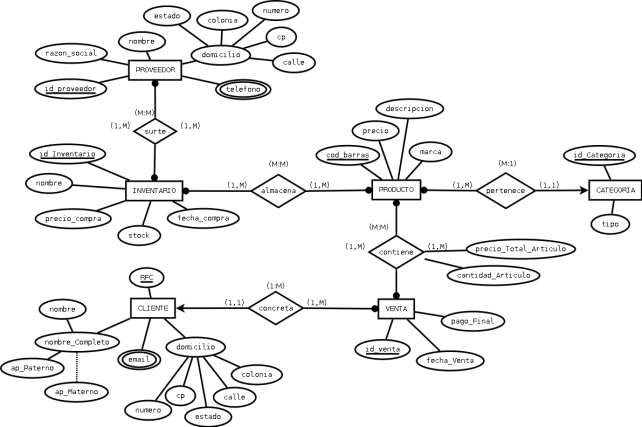
\includegraphics[width=\linewidth]{img/MER}
				\caption{Modelo Entidad-Relación.}
			\end{figure}
			
			
		\subsection{Modelo lógico}
			\subsubsection{Representación Intermedia}
				Realizando el Modelo Entidad-Relación, pudimos seguir las reglas para de la transformación de
				MER a MR, nos derivó en las siguientes tablas:
				
			\begin{itemize}
				\item PROVEEDOR: \{ id\_proveedor smallint (PK), nombre varchar 50, razón social varchar 50, estado varchar 50, colonia varchar 50, numero smallint, cp smallint, calle varchar 50\}
				\item TELEFONO: \{teléfono bigint(PK), id\_proveedor smallint (FK)\}
				
				\item INVENTARIO: \{id\_Inventario smallint (PK), precio\_compra decimal (10,2), stock smallint, fecha\_compra date \}
				
				\item SURTE: \{[id\_Provedor smaillint (FK), id\_Inventario smallint (FK)] (PK)\}
				
				\item PRODUCTO: \{cod\_barras integer PK, id\_categoria smallint FK, precio smallint NOT NULL, marca varchar(20) NOT NULL, descripcion varchar(50), id\_inventario smallint (FK)\}
				
				\item CATEGORÍA: \{ id\_categoria smallint PK, tipo varchar(20) NOT NULL\}
				
				\item CLIENTE: \{RFC varchar(13) (PK), nombre varchar(20), ap\_paterno varchar (20), ap\_materno varchar (20) (N), cp smallint, numero smallint, estado varchar (32), calle varchar (32), colonia varchar (32)\}
				
				\item EMAIL: \{RFC varchar(13) (FK), email varchar (64) (PK)\}
				
				\item VENTA: \{id\_venta int(PK), fecha\_venta date, pago\_final decimal(7,2), RFC varchar(13)(FK)\}
				
				\item CONTIENE: \{ [cod\_barras int , id\_venta int](PK)(FK), precioTotalArt decimal(7,2), cantidad articulo int\} 
			\end{itemize}
			
			\subsubsection{Transformación de MER a MR}
				Para la transformación de Modelo Entidad Relación a Modelo Relacional, primero debemos utilizar la transformación intermedia que obtuvimos y desarrollamos. Una vez finalizado ese procedimiento utilizamos las reglas para la trasformación de MER a MR y obtendremos nuestro modelo relacional.
			\subsubsection{Modelo Relacional}
			
			\subsubsection{Normalización}
		
	\section{Implementación}
		Para llevar a cabo la implementación de esta base de datos, primero tendremos que crear la base de datos en el manejador POSTGRESQL.8 Una vez finalizada la creación de la base de datos, tendremos que crear las tablas que obtuvimos en nuestro modelo relacional. Estas tablas tendrán que tener sus respectivos constraints para las
		llevas primarias y foráneas que se utilizan en toda la base de datos. Cuando las tablas estén creadas en las base de datos, podremos verificar su utilidad haciendo
		inserciones de prueba. Para que el sistema resuelva cuando se reciba un código de barras regrese la utilidad, para que cuando haya la venta de un artículo y se decremente el stock por la cantidad vendida, dada una fecha o una fecha de inicio y de fin, regrese la cantidad total que se vendió y su ganancia correspondiente. Para obtener el nombre de aquellos productos que están es stock, que de forma	automática genere vista que contenga información para desplegar una factura de compra y la creación del índice. Para todas esas funciones mencionadas, tendremos que hacer uso de la creación de Functions, Procedures y Triggers.
		
		\subsection{Modelo físico}
			Para el desarrollo de la base de datos y su implementación, tendremos que trabajar con la creación de tablas y sus respectivas inserciones en el manejador, tendremos que utilizar la programación en base de datos para que se logren hacer las funciones que se nos solicitan. Lo primero que realizamos fue la creación de tablas, que a su vez son las mismas que obtuvimos del Modelo Relacional, las tablas que creamos son las que se ilustran a continuación:
		
		%imagenes
		
		También para comprobar que la creación de estas tablas fue correcta, tuvimos que realizar inserciones que tuvieran relación con estas tablas. Las inserciones que realizamos son las siguientes:
		
		%imagenes
		
		Para lograr obtener las funciones solicitadas en los requerimientos, tendremos que utilizar la programación en base de datos. Lo que realizamos fue para cada uno de los puntos que tenemos en los requerimientos. Cabe aclarar que estas funciones, luego tendrán que ir acompañadas de triggers, para que al momento de usar estas funciones, sea de manera inmediata.
		Función que retorna la utilidad.
		- El primer requerimiento de las funcione nos pide que al recibir un código de barras de un producto, este regrese la utilidad, en este caso la utilidad represente el precio al que el producto es ofertado menos el precio al que el producto fue adquirido al proveedor.
		
		%imagen
		
		Las siguientes Functions, representan al requerimiento que nos solicita dada una fecha, o fecha de inicio y fecha de fin se nos solicita regresar la cantidad del total que se vendió y la ganancia correspondiente.
		
		Función para retornar pagos finales
		
		%imagen
		
		Función para retornar pagos finales entre fechas
		
		%imagen
		
		Función para retornar las ganancias
		
		%imagen
		
		Función para retornar las ganancias por fechas
		
		%imagen
		
		
		
			\subsubsection{IaaS}
	
		\subsection{Códigos}
		
		\subsection{DDL}
	
	\section{Presentación}
		Una interfaz gráfica es un programa que nos permite manipular información a través de objetos gráficos que proporcionen un entorno visual, con el fin facilitar la interacción del usuario con la computadora.\par
		En este caso, se optó por desarrollar una página web como interfaz gráfica que permita la manipulación de información de nuestra base de datos.
		
		\subsection{Django}
		Django es un framework de Python de alto nivel que permite diseñar aplicaciones web de una forma rápida, limpia y pragmática. Además, ayuda a los desarrolladores a evitar muchos errores de seguridad comunes, como la inyección de SQL, las secuencias de comandos entre sitios, la falsificación de solicitudes entre sitios y el secuestro de clics.
			
			\subsubsection{Mapeo Relacional de Objetos}
			El Mapeo Relacional de Objetos o ORM (\textit{Object Relational Mapping}), es una tecnología que soluciona el desajuste entre las bases de datos relacionales y orientadas a objetos.\par 
			Por lo general, asigna una clase a una tabla uno a uno. Cada instancia de la clase corresponde a un registro en la tabla y cada atributo de la clase corresponde a cada campo en la tabla. ORM proporciona una asignación a la base de datos, en lugar de escribir código SQL directamente, solo es necesario manipular los datos de la base de datos como un objeto operativo.\par 
			Si bien, el ORM es una herrmienta muy util, no se utilizará en este proyecto, ya que preferimos escribir directamente la sentencia SQL para comunicarnos con la base de datos.
			
			\subsubsection{Ejecutar SQL personalizado directamente}
			El objeto \textbf{django.db.connection} representa la conexión por defecto entre django y la base de datos. Las funciones que utilizamos para la comunicación con la base de datos son las siguientes:
			\begin{itemize}
				\item \textbf{connection.cursor()}
					\subitem Para obtener un objeto cursor.
					
				\item \textbf{cursor.execute(sql, [params])}
					\subitem Para ejecutar sentencias SQL.
					
				\item \textbf{cursor.fetchall()}
					\subitem Para devolver las filas resultantes de la consulta.
			\end{itemize}
		
		\subsection{Diseño}
		
	
	\section{Conclusiones}
		\begin{itemize}
			\item 
				\subitem 
				
			\item López González Kevin
				\subitem Bla bla bla

			\item 
				\subitem
		\end{itemize}

	
\end{document}



















